\documentclass[a4paper]{article}

\usepackage[T1]{fontenc}
\usepackage{titling}
\usepackage[polish]{babel}
\usepackage{multirow}
\selectlanguage{polish}
\usepackage[utf8]{inputenc}
\usepackage{amsmath}
\usepackage{listings}
\usepackage{graphicx}
\usepackage{framed}
\usepackage{fullpage}
\usepackage{adjustbox}
\usepackage{algpseudocode}


\setlength{\droptitle}{+10em}
\title{\huge
  Obliczenia naukowe \\
  \large Lista 3}
\author{Arkadiusz Ziobrowski \\ 229728}
\date{}

\begin{document}
\maketitle

\pagebreak




\section{Zadanie pierwsze}

\subsection{Opis problemu}
\paragraph{}
Celem zadania była implementacja funkcji, rozwiązującej równanie $f(x) = 0$ metodą bisekcji.
\subsection{Rozwiązanie}
\paragraph{}
W języku programowania \texttt{Julia} została zaimplementowana funkcja o następującej sygnaturze:
\begin{center}
\texttt{function mbisekcji(f, a::Float64, b::Float64, delta::Float64, epsilon::Float64)},
\end{center}

gdzie \texttt{f} to funkcja $f(x)$ zadana jako funkcja anonimowa, \texttt{a} oraz \texttt{b} to końce przedziału początkowego, zaś \texttt{delta} i \texttt{epsilon} to żądane dokładności obliczeń. Funkcja powinna zwracać czwórkę uporządkowaną \texttt{(r, v, it, err)}, gdzie \texttt{r} to przybliżenie pierwiastka równania $f(x) = 0$, \texttt{v} to wartość $f(r)$, \texttt{it} to liczba wykonanych iteracji, a \texttt{err} to sygnalizacja błędu, który nastąpił w trakcie obliczeń.

\paragraph{}
\begin{center}
	\begin{algorithmic}[1]
	\Function{mbisekcji}{$f$, $a$, $b$, $\delta$, $\epsilon$}
    	\State $u\gets f(a)$
    	\State $v\gets f(b)$
    	\State $e\gets b - a$
    	\If {$sgn(u) = sgn(v)$}
    		\State \Return error
    	\EndIf
    	\State $e\gets e / 2$
    	\State $c\gets a + e$
    	\State $w\gets f(c)$
    	\While{$|e| > \delta \land |w| > \epsilon$}
    		\If{$sgn(w) \neq sgn(u)$}
    			\State $b\gets c$
    			\State $v\gets w$
    		\Else
    			\State $a\gets c$
    			\State $u\gets w$
    		\EndIf
    		\State $e\gets e / 2$
    		\State $c\gets a + e$
    		\State $w\gets f(c)$
    	\EndWhile
    	\State \Return ($c$, $w$, $it$, $err$)
	\EndFunction
	\end{algorithmic}
\end{center}

Powyższy pseudokod prezentuje algorytm bisekcji. Metoda bisekcji polega na połowieniu przedziału początkowego i wyborze lokalizacji miejsca zerowego w dwóch podziałach przy pomocy funkcji $sgn$. W liniach 5-7 następuje sprawdzenie czy wartości funkcji na krańcach przedziału początkowego mają różne znaki. W liniach 8-10 wyznaczamy punkt środkowy i wyliczamy odpowiadającą mu wartość funkcji $f$. Następnie iterujemy aż do momentu, gdy spełnione jest przynajmniej jedno z żądanych przez nas kryteriów, czyli gdy błąd jest wystarczająco mały lub wartości funkcji $f$ w punkcie środkowym jest bliska zeru. W liniach 12-18 podejmowana jest decyzja, w której części połowionego przedziału znajduje się miejsce zerowe. Na mocy własności Darboux, jeśli funkcja jest ciągła w przedziale $[a, b]$ i zmienia w nim znak, to funkcja ta musi mieć zero w $(a, b)$. Sprawdzamy zatem, czy znak funkcji zmienia sie dla $f(a)$ i $f(c)$ oraz dla $f(c)$ i $f(b)$. Zmiana znaku dla $f(a)$ i $f(c)$ pokazuje, że miejsce zerowe znajduje się w przedziale $[a, c]$. W linii 13 nadpisujemy przedział nową wartością. Dla $sgn(f(c)) \neq sgn(f(b))$ postępujemy analogicznie. W liniach 19-21 ponownie wyznaczamy punkt środkowy, tak samo jak w liniach 8-10.

\paragraph{Zastosowane rozwiązania}
W algorytmie zostało zastosowanych kilka rozwiązań, do których warto dodać krótki komentarz. Do rozpoznawania znaku funkcji została użyta funkcja $sgn$, ponieważ zastosowanie $f(a)*f(c) < 0$ wprowadza zbędne mnożenie, które ponadto może powodować nadmiar lub niedomiar. Również wyznaczanie środka przedziału jako $a + e/2$, zamiast $(a + b)/2$ pozwala uniknąć błędów. Wartości \texttt{err} w czwórce uporządkowanej \texttt{(r, v, it, err)} służą jako flagi błędów dla metody bisekcji. W implementacji w języku \texttt{Julia} mogą przyjmować wartości odpowiadające błędom braku zmiany znaku, nieprawidłowych argumentów funkcji, bądź też wskazujące na poprawne działanie algorytmu.

\section{Zadanie drugie}

\subsection{Opis problemu}
\paragraph{}
Celem zadania była implementacja funkcji, rozwiązującej równanie $f(x) = 0$ metodą Newtona.

\subsection{Rozwiązanie}
\paragraph{}
W języku programowania \texttt{Julia} została zaimplementowana funkcja o następującej sygnaturze:
\begin{center}
\texttt{function mstycznych(f, pf, x0::Float64, delta::Float64, epsilon::Float64, maxit::Int)},
\end{center}

gdzie \texttt{f} to funkcja $f(x)$ zadana jako funkcja anonimowa, \texttt{pf} to pochodna funkcji $f(x)$ zadana jako funkcja anonimowa, \texttt{x0} to przybliżenie początkowe, zaś \texttt{delta} i \texttt{epsilon} to żądane dokładności obliczeń, a \texttt{maxit} to maksymalna dopuszczalna liczba iteracji. Funkcja powinna zwracać czwórkę uporządkowaną \texttt{(r, v, it, err)}, gdzie \texttt{r} to przybliżenie pierwiastka równania $f(x) = 0$, \texttt{v} to wartość $f(r)$, \texttt{it} to liczba wykonanych iteracji, a \texttt{err} to sygnalizacja błędu, który nastąpił w trakcie obliczeń.

\paragraph{}
\begin{center}
	\begin{algorithmic}[1]
	\Function{mstycznych}{$f$, $pf$, $x_{0}$, $\delta$, $\epsilon$, $maxit$}
    	\State $v\gets f(x_{0})$
    	\If {$|v| < \epsilon$}
    		\State \Return ($x_{0}$, $v$, $it$, $err$)
    	\EndIf
    	\For{$k = 1$ \textbf{to} $maxit$}
    		\If{$|pf(x_{0})| < macheps$}
    			\State \Return error
    		\EndIf
    		\State $x_{1}\gets x_{0} - v / f'(x_{0})$
    		\State $v\gets f(x_{1})$
    		\If{$|x_{1} - x_{0}| < \delta \lor |v| < \epsilon$}
    			\State \Return ($x_{1}$, $v$, $it$, $err$)
    		\EndIf
    		\State $x_{0}\gets x_{1}$
    	\EndFor
    	\State \Return error
	\EndFunction
	\end{algorithmic}
\end{center}

Powyższy pseudokod prezentuje algorytm Newtona. Polega on na rekurencyjnym zastosowaniu wzoru $x_{n+1} = x_{n} - f(x_{n}) / f'(x_{n})$, zaczynając od $x_{0}$, będącego przybliżeniem zera $r$. W linii 2 liczymy wartość funkcji dla zadanego przybliżenia, a następnie sprawdzamy, czy nie osiągnęliśmy zadanej precyzji wartości funkcji. Iterujemy aż do spełnienia warunków w linii 12 lub osiągnięcia maksymalnej liczby iteracji. W liniach 7-9 wartość pochodnej funkcji $f$ w punkcie $x_{0}$ jest porównywana z wartością bliską zeru. W przypadku, gdy tak jest zwracamy błąd, gdyż funkcja nie będzie zbieżna do interesującego nas wyniku, bądź będzie zbiegać zbyt wolno. W linii 10 zastosowany został podany wcześniej wzór rekurencyjny. W liniach 12-13 sprawdzamy, czy różnica między punktem $x_{0}$, a $x_{1}$ jest mniejsza od zadanej $\delta$ lub czy wartość funkcji dla punktu $x_{1}$ co do wartości bezwzględnej jest mniejsza od zadanego $\epsilon$.

\paragraph{Zastosowane rozwiązania}
Podobnie jak w przypadku metody bisekcji, wartości \texttt{err} w czwórce uporządkowanej \texttt{(r, v, it, err)} służą jako flagi błędów dla metody Newtona. W implementacji w języku \texttt{Julia} mogą przyjmować wartości odpowiadające błędom przekroczenia maksymalnej liczby iteracji, nieprawidłowych argumentów funkcji, bądź też wskazujące na poprawne działanie algorytmu.

\section{Zadanie trzecie}

\subsection{Opis problemu}
\paragraph{}
Celem zadania była implementacja funkcji, rozwiązującej równanie $f(x) = 0$ metodą siecznych.

\subsection{Rozwiązanie}
\paragraph{}
W języku programowania \texttt{Julia} została zaimplementowana funkcja o następującej sygnaturze:
\begin{center}
\texttt{function msiecznych(f, x0::Float64, x1::Float64, delta::Float64, epsilon::Float64, maxit::Int)},
\end{center}

gdzie \texttt{f} to funkcja $f(x)$ zadana jako funkcja anonimowa, \texttt{x0} i \texttt{x1} to przybliżenia początkowe, zaś \texttt{delta} i \texttt{epsilon} to żądane dokładności obliczeń, a \texttt{maxit} to maksymalna dopuszczalna liczba iteracji. Funkcja powinna zwracać czwórkę uporządkowaną \texttt{(r, v, it, err)}, gdzie \texttt{r} to przybliżenie pierwiastka równania $f(x) = 0$, \texttt{v} to wartość $f(r)$, \texttt{it} to liczba wykonanych iteracji, a \texttt{err} to sygnalizacja błędu, który nastąpił w trakcie obliczeń.

\paragraph{}
\begin{center}
	\begin{algorithmic}[1]
	\Function{msiecznych}{$f$, $x_{0}$, $x_{1}$, $\delta$, $\epsilon$, $maxit$}
    	\State $fx_{0}\gets f(x_{0})$
    	\State $fx_{1}\gets f(x_{1})$
    	\For{$k = 1$ \textbf{to} $maxit$}
    		\If{$|fx_{0}| > |fx_{1}|$}
    			\State swap($x_{0}$, $x_{1}$)
    			\State swap($fx_{0}$, $fx_{1}$) 
    		\EndIf
    		\State $s\gets (x_{1} - x_{0}) / (fx_{1} - fx_{0})$
    		\State $x_{1}\gets x_{0}$
    		\State $fx_{1}\gets fx_{0}$
    		\State $x_{0}\gets x_{0} - fx_{0} * s$
    		\State $fx_{0}\gets f(x_{0})$
    		\If{$|x_{1} - x_{0}| < \delta \lor |fx_{0}| < \epsilon$}
    			\State \Return ($x_{1}$, $v$, $it$, $err$)
    		\EndIf
    	\EndFor
    	\State \Return error
	\EndFunction
	\end{algorithmic}
\end{center}

Powyższy pseudokod prezentuje algorytm siecznych. Polega on na zastosowaniu zmodyfikowanego wzoru rekurencyjnego z metody Newtona, który ma następującą postać: $x_{n+1} = x_{n} - f(x_{n}) * (x_{n} - x_{n-1}) / (f(x_{n}) - f(x_{n-1}))$. Iterujemy dopóki nie zajdą warunki w linii 14, bądź nie osiągniemy maksymalnej liczby iteracji. W liniach 5-8 zamieniamy $x_{0}$ i $x_{1}$ oraz odpowiadające im wartości funkcji, gdy nie jest utrzymana nierówność $|f(x_{0})| \leq |f(x_{1})|$. Jest to niezbędne do zachowania poprawnej formy równania rekurencyjnego. W liniach 9-13 zastosowany jest podany wcześniej wzór rekurencyjny. W liniach 14-16 sprawdzamy, czy różnica między punktem $x_{0}$, a $x_{1}$ jest mniejsza od zadanej $\delta$ lub czy wartość funkcji dla punktu $x_{0}$ co do wartości bezwzględnej jest mniejsza od zadanego $\epsilon$.

\paragraph{Zastosowane rozwiązania}
Podobnie jak w przypadku metody Newtona, wartości \texttt{err} w czwórce uporządkowanej \texttt{(r, v, it, err)} służą jako flagi błędów dla metody siecznych. W implementacji w języku \texttt{Julia} mogą przyjmować wartości odpowiadające błędom przekroczenia maksymalnej liczby iteracji, nieprawidłowych argumentów funkcji, bądź też wskazujące na poprawne działanie algorytmu. Metoda siecznych jest bardziej efektywna od metody Newtona pod względem ilości wykonanych obliczeń. W metodzie Newtona niezbędne było obliczenie pochodnej funkcji $f$, natomiast w metodzie siecznych wystarczające jest obliczenie dwóch punktów $x_{n}$ oraz $x_{n-1}$, a w kolejnych krokach algorytmu dla $x_{n+1}$ tylko jednej nowej wartości funkcji $f$. Dlatego też algorytm siecznych może być w pewnych przypadkach szybszy od metody Newtona, mimo że jego nadliniowa zbieżność jest nieco wolniejsza niż kwadratowa zbieżność algorytmu Newtona.

\section{Zadanie czwarte}

\subsection{Opis problemu}
\paragraph{}
Celem zadania było wyznaczenie pierwiastka równania $sin(x) - (\frac{1}{2}x)^2 = 0$ przy użyciu metod zaprogramowanych w zadaniu pierwszym, drugim oraz trzecim. Dla każdej z metod zostały podane parametry wywołania.

\subsection{Rozwiązanie}
\paragraph{}
W zadaniu zostały wykorzystane zaimplementowane wcześniej w języku programowania \texttt{Julia} funkcje, będące realizacjami metod bisekcji, stycznych i siecznych. Funkcje te zostały umieszczone w module \texttt{EquationSolving}, który musi zostać zaimportowany do programu przy pomocy instrukcji \texttt{using}, aby było możliwe korzystanie z wymienionych funkcji. Metody znajdowania pierwiastka zadanego równania zostały wywołane z następującymi argumentami:

\begin{center}
\begin{itemize}
\item	Metoda bisekcji z przedziałem początkowym $[1.5, 2]$, $\delta = \frac{1}{2}10^{-5}$ i $\epsilon = \frac{1}{2}10^{-5}$.
\item	Metoda Newtona z przybliżeniem początkowym $x_{0} = 1.5$, $\delta = \frac{1}{2}10^{-5}$ i $\epsilon = \frac{1}{2}10^{-5}$.
\item	Metoda siecznych z przybliżeniami początkowymi $x_{0} = 1.5$, $x_{1} = 2.0$, $\delta = \frac{1}{2}10^{-5}$ i $\epsilon = \frac{1}{2}10^{-5}$.
\end{itemize}
\end{center}

\subsection{Wyniki i interpretacja}
\paragraph{}

\begin{center}
 \begin{tabular}{ |c | c | c | c | c|  }
 \hline
   & Miejsce zerowe $x$ & Wartość $f(x)$ & Liczba iteracji & Flaga błędu\\
 \hline
 Metoda bisekcji & 1.9337539672851562 & -2.7027680138402843e-7 & 16 & 0 \\
 Metoda Newtona & 1.933753779789742 & -2.2423316314856834e-8 & 4 & 0 \\
 Metod siecznych & 1.933753644474301 & 1.564525129449379e-7 & 4 & 0 \\ 
 \hline
\end{tabular}
\end{center}

W powyższej tabeli zostały przedstawione wyniki wywołań funkcji dla zadanych argumentów. Metoda Newtona dała najbardziej dokładny co do wartości $f(x)$ wynik w stosunkowo małej liczbie iteracji. Mała liczba iteracji metody Newtona wynika z jej kwadratowej zbieżności. Cztery iteracje wykonała również metoda siecznych, dając jednak mniej dokładny wynik. Najmniej dokładny wynik uzyskała metoda bisekcji, kończąca swoje działanie po trzynastu iteracjach. Taka ilość iteracji wynika z liniowej zbieżności metody bisekcji.

\paragraph{}
Dla dobranych danych warto również przeanalizować działanie funkcji w kontekście czasu wykonania. Pozwoli to na porównanie szybkości metody Newtona i metody siecznych, które wykonały się jednakową liczbę iteracji. 

\begin{center}
 \begin{tabular}{ |c | c | c|  }
 \hline
   & Czas (w sekundach) & Liczba iteracji\\
 \hline
 Metoda bisekcji & 0.017236463 & 13 \\
 Metoda Newtona & 0.019736448 & 4 \\
 Metod siecznych & 0.015185165 & 4 \\ 
 \hline
\end{tabular}
\end{center}

Powyższa tabela pokazuje, że intuicje wiążące mniejszą liczbę iteracji z szybszym czasem wykonywania nie zawsze są poprawne\footnote{Wyniki otrzymane przy użyciu funkcji \texttt{tic()} oraz \texttt{toc()} z języka \texttt{Jullia} zostały uśrednione, jednak dla tak szybkich wykonań zawierają narzut pracy procesora.}. Metoda bisekcji z trzynastoma iteracjami wykonała się szybciej niż metoda Newtona z jedynie czterema iteracjami. Spowodowane to jest koniecznością obliczenia wartości pochodnej w algorytmie Newtona, co przekłada się na czasy wykonania. Tabela ta rozstrzyga również szybkość wykonania na korzyść metody siecznych w stosunku do metody Newtona. Metoda siecznych wykonuje się szybciej, gdyż nie wymaga obliczania pochodnej funkcji i w każdej iteracji musi obliczyć tylko jedną wartość funkcji (z wyjątkiem pierwszej, gdy są obliczane wartości $f(x_{0})$ i $f(x_{1})$).

\subsection{Wnioski}
\paragraph{}
Metody bisekcji, Newtona i siecznych dają zbliżone wyniki dla miejsc zerowych do 4 miejsca po przecinku. Różnią się jednak dokładnością wyniku i szybkością działania. Dobór odpowiedniej metody pozwala rozstrzygnąć konflikt między szybkością, a wiarygodnością programu. Dla zadanych w tym problemie argumentów najbardziej wiarygodną metodą jest metoda Newtona, zaś najszybszą (choć również zapewniającą zadowalający wynik) jest metoda siecznych.


\section{Zadanie piąte}

\subsection{Opis problemu}
\paragraph{}
Celem zadania było wyznaczenia takich $x$, dla których przecinają się wykresy funkcji $y_{1} = 3x$ i $y_{2} = e^x$. Do zadania miała zostać użyta metoda bisekcji z podanymi parametrami dokładności obliczeń.

\subsection{Rozwiązanie}
\paragraph{}
W zadaniu została wykorzystana zaimplementowana wcześniej w języku programowania \texttt{Julia} funkcja, będąca realizacją metody bisekcji. Funkcja ta znajduje się w module \texttt{EquationSolving}, który musi zostać zaimportowany do programu przy pomocy instrukcji \texttt{using}, aby możliwe było wywołanie wymienionej funkcji. Metoda bisekcji została wywołana z parametrami dokładności $\delta = 10^{-4}$ i $\epsilon = 10^{-4}$.

W miejscu przecięciu wykresów funkcje mają taką samą wartość. Korzystając z tej własności stworzyłem nową funkcję $y = y_{1} - y_{2} = 3x - e^x$. Miejsca zerowe nowej funkcji $y$ będą miejscami przecięć wykresów funkcji $y_{1}$ i $y_{2}$.

\paragraph{}
\begin{figure}[htbp]
  \centering
  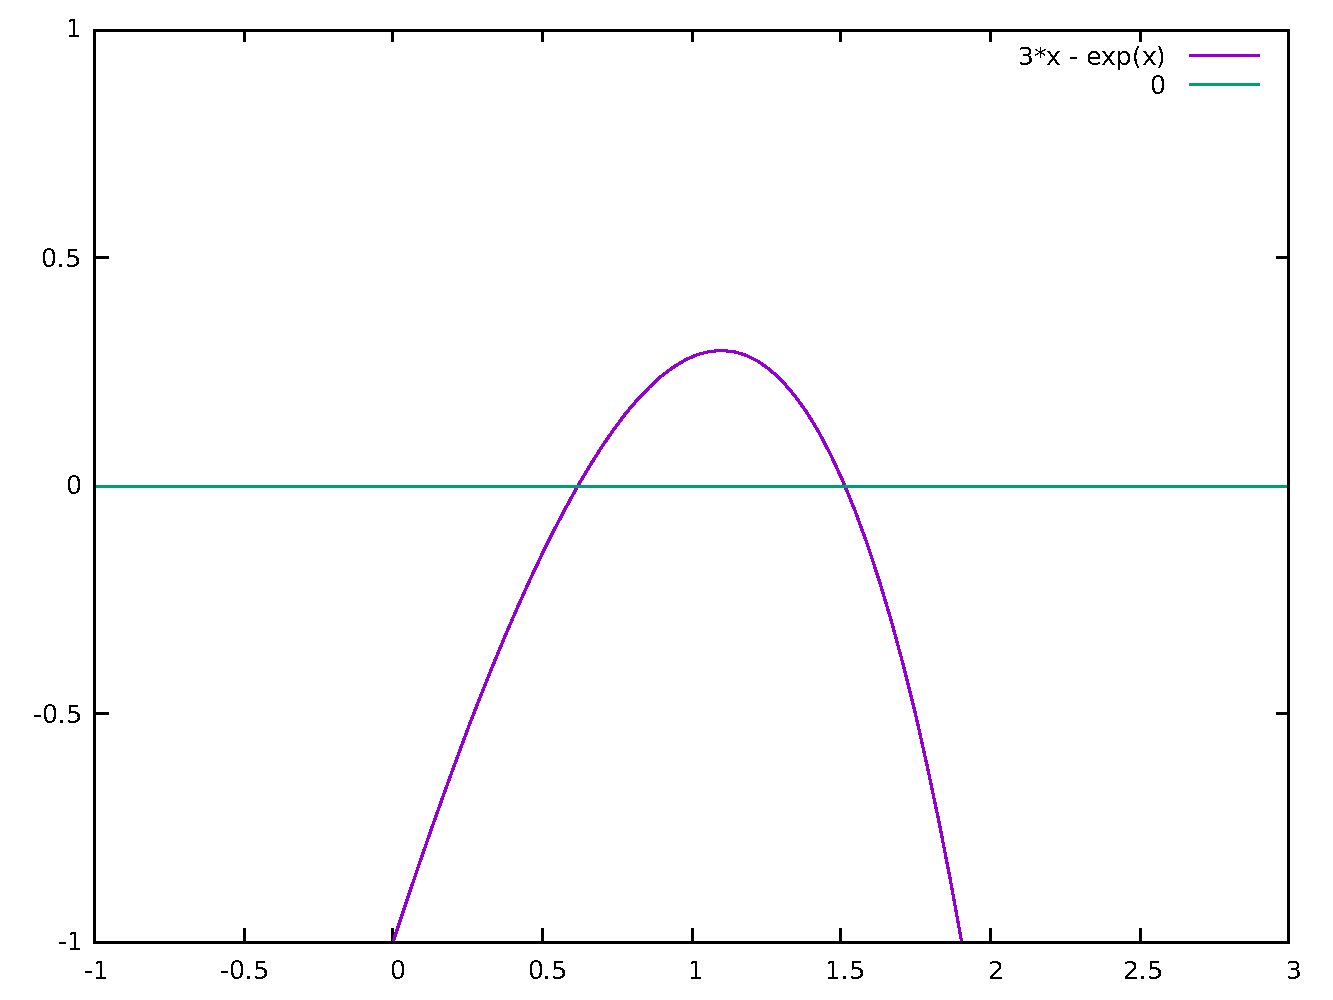
\includegraphics[scale=0.35]{wykres.pdf}
  \caption{Wykres dla funkcji $y = 3x - e^x$ stworzony przy użyciu narzędzia \textit{gnuplot}}
\end{figure}

Aby wyznaczyć miejsca zerowe nowej funkcji $y$ stworzyłem jej wykres, a następnie określiłem przedziały, w których znajdują się miejsca zerowe. Dla znalezionych przedziałów wywołałem funkcję odpowiadającą metodzie bisekcji z przedziałem i zadanymi dokładnościami jako argumentami.

\subsection{Wyniki i interpretacja}
\paragraph{}

\begin{center}
 \begin{tabular}{ |c | c | c | c|  }
 \hline
  Przedział & Miejsce zerowe $x$ & Wartość $f(x)$ & Liczba iteracji\\
 \hline
 $[0.0, 1.0]$ & 0.619140625 & 9.066320343276146e-5 & 9\\
 $[1.0, 2.0]$ & 1.51171875 & 0.000638447089475136 & 8 \\
 \hline
\end{tabular}
\end{center}

Obydwa wywołania funkcji kończą się z flagą błędu \texttt{BISECTION\_NO\_ERR} (wartość zero), która sygnalizuje prawidłowe wykonanie algorytmu. Widoczne jest zatem, że przy doborze odpowiednich przedziału metoda bisekcji znajdzie miejsca zerowe funkcji w tych przedziałach. Jest to ważna własność metody bisekcji, gdyż metody Newtona i siecznych mogą dla pewnych danych rozbiegać od prawidłowego wyniku.


\subsection{Wnioski}
\paragraph{}
Metoda bisekcji pozwala na znalezienie miejsc zerowych w podanych przedziałach z zadaną dokładnością, jeżeli miejsca zerowe faktycznie się w nich znajdują. Żeby znaleźć przedziały, w których znajdują się miejsca zerowe warto jest znaleźć wykres funkcji i na jego podstawie dobrać parametry wejściowe.

\section{Zadanie szóste}

\subsection{Opis problemu}
\paragraph{}
Celem zadania było znalezienie miejsc zerowych funkcji $f_{1}(x) = e^{1 - x} - 1$ oraz $f_{2}(x) = xe^{-x}$ za pomocą metod bisekcji, Newtona i siecznych. Należało dla zadanych dokładności dobrać odpowiednie przedziały i przybliżenia początkowe. Następnie należało przeprowadzić serię eksperymentów pokazujących zachowanie metody Newtona w zależności od doboru przybliżeń początkowych.

\subsection{Rozwiązanie}
\paragraph{}
W zadaniu zostały wykorzystane zaimplementowane wcześniej w języku programowania \texttt{Julia} funkcje, będące realizacjami metod bisekcji, stycznych i siecznych. Funkcje te zostały umieszczone w module \texttt{EquationSolving}, który musi zostać zaimportowany do programu przy pomocy instrukcji \texttt{using}, aby było możliwe korzystanie z wymienionych funkcji.

Podobnie jak w przypadku zadania piątego należało tutaj dobrać odpowiednie parametry dla wywołań funkcji, czyli przybliżenia początkowe dla metod Newtona i siecznych oraz przedziały dla metody bisekcji. Dla wszystkich metod zostały zadane dokładności $\delta = 10^{-5}$ i $\epsilon = 10^{-5}$. Maksymalna liczba iteracji w metodach Newtona i siecznych to czterdzieści.

\paragraph{}
\begin{figure}[htbp]
  \centering
  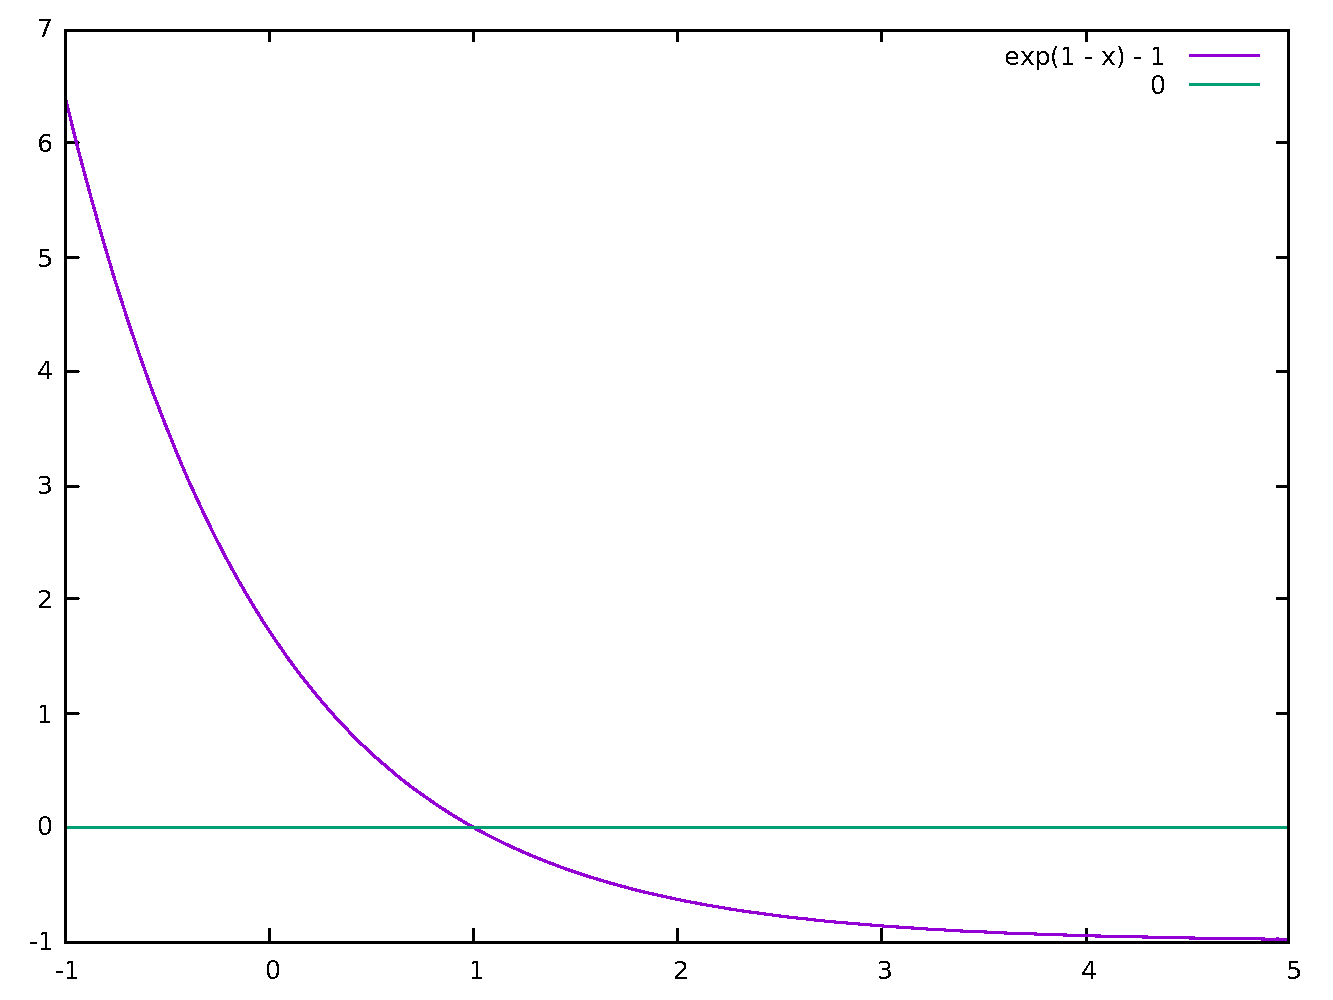
\includegraphics[scale=0.35]{wykres6a.pdf}
  \caption{Wykres dla funkcji $f_{1}(x) = e^{1 - x} - 1$ stworzony przy użyciu narzędzia \textit{gnuplot}}
\end{figure}
\clearpage

Na podstawie wykresu można stwierdzić, że miejsce zerowe funkcji znajduje się w okolicach liczby jeden. Będziemy zatem dobierać parametry wywołania dla funkcji $f_{1}(x) = e^{1 - x} - 1$ następująco:

\begin{center}
\begin{itemize}
\item Dla metody bisekcji dobór przedziału $[a, b]$, gdzie między wartościami $a$ i $b$ znajduje się liczba jeden.
\item Dla metody Newtona dobór przybliżenia początkowego $x_{0}$ blisko jedynki, jednakże należy mieć na uwadze spłaszczenie funkcji $f_{1}$, do którego wyznaczone styczne przecinające się z osią $X$ będą nas oddalały od miejsca zerowego. Należy również zwrócić uwagę na osiąganie przez pochodną wartości bliskich zeru w spłaszczonej części funkcji.
\item Dla metody siecznych musimy uważać, aby wzięte przybliżenia początkowe dawały sieczną, przecinającą oś $X$. Musimy również wziąć punkty odpowiednio blisko miejsca zerowego, gdyż w przeciwnym wypadku metoda siecznych może nie zbiegać do rozwiązania.
\end{itemize}
\end{center}

\paragraph{}
\begin{figure}[htbp]
  \centering
  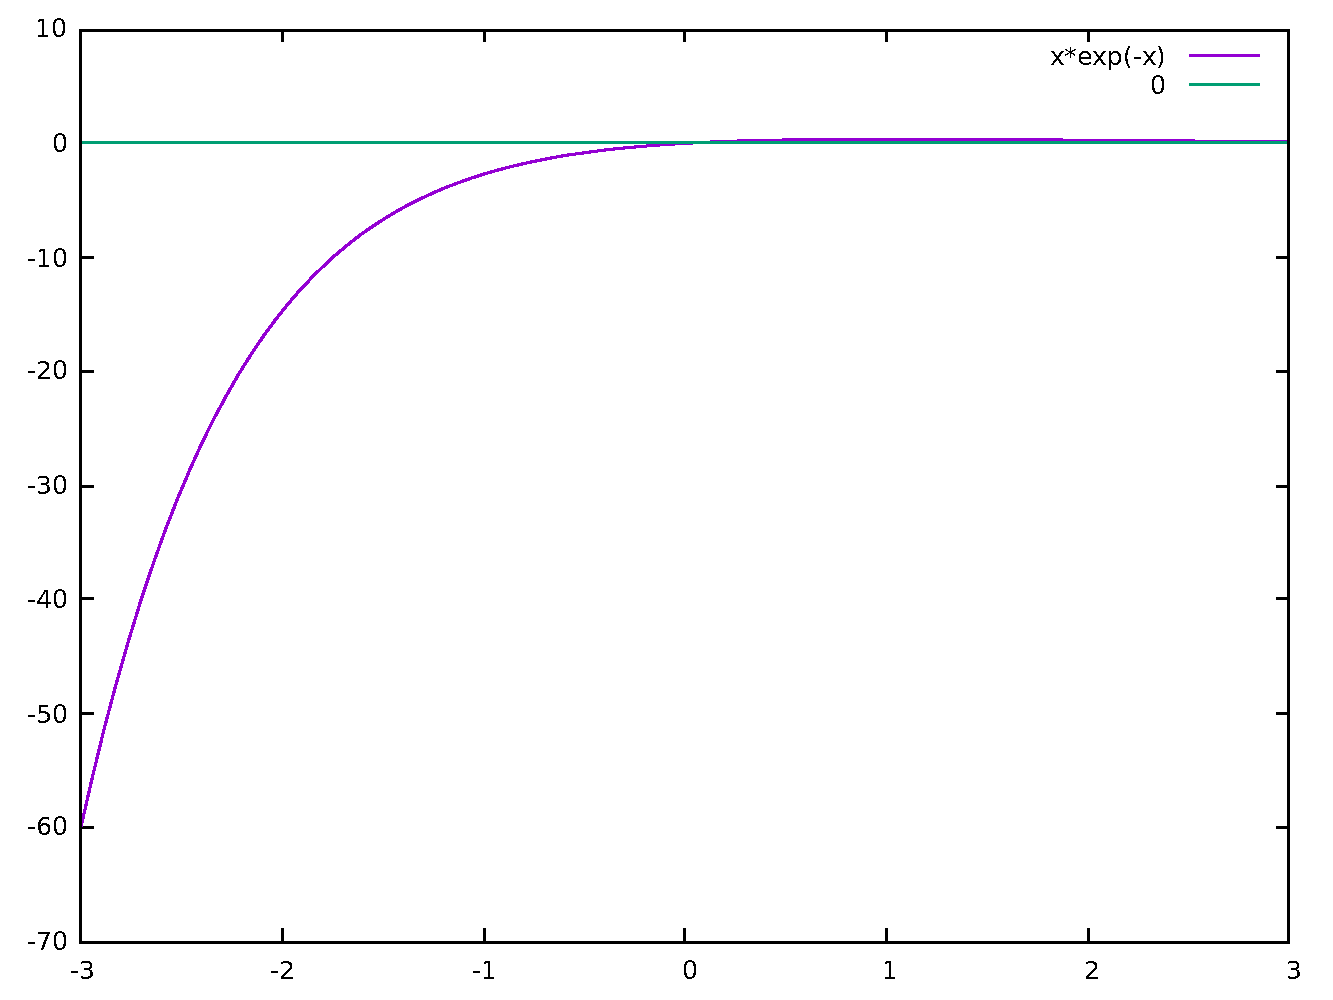
\includegraphics[scale=0.35]{wykres6b.pdf}
  \caption{Wykres dla funkcji $f_{2}(x) = xe^{-x}$ stworzony przy użyciu narzędzia \textit{gnuplot}}
\end{figure}

Na podstawie wykresu można stwierdzić, że miejsce zerowe funkcji znajduje się w okolicach liczby zero. Będziemy zatem dobierać parametry wywołania dla funkcji $f_{2}(x) = xe^{-x}$ następująco:

\begin{center}
\begin{itemize}
\item Dla metody bisekcji dobór przedziału $[a, b]$, gdzie między wartościami $a$ i $b$ znajduje się liczba zero.
\item Dla metody Newtona dobór przybliżenia początkowego $x_{0}$ blisko zera, jednakże należy mieć na uwadze spłaszczenie funkcji $f_{1}$, do którego wyznaczone styczne przecinające się z osią $X$ będą nas oddalały od miejsca zerowego, bądź też wprowadzą nas zbyt szybko w zadaną dokładność. Należy również zwrócić uwagę na osiąganie przez pochodną wartości bliskich zeru w spłaszczonej części funkcji.
\item Dla metody siecznych musimy uważać, aby wzięte przybliżenia początkowe dawały sieczną, przecinającą oś $X$. Musimy również wziąć punkty odpowiednio blisko miejsca zerowego, gdyż w przeciwnym wypadku metoda siecznych może nie zbiegać do rozwiązania.
\end{itemize}
\end{center}
\clearpage

\subsection{Wyniki i interpretacja}
\paragraph{}
\begin{center}
 \begin{tabular}{ |c | c | c | c | c|  }
 \hline
 \multicolumn{5}{|c|}{$f_{1}(x) = e^{1 - x} - 1$} \\
 \hline
 & Dane wejściowe & Miejsce zerowe $x$ & Wartość $f(x)$ & Liczba iteracji\\
 \hline
 Metoda bisekcji & $[0.0, 2.0]$ & 1.0 & 0.0 &  1\\
 Metoda bisekcji & $[0.0, 1.5]$ & 0.99993896484375 & 6.103701893311886e-5 & 13\\
 Metoda Newtona & $x_{0} = 7.5$ & -617.6416330443619 & 4.7059521480000026e268 & 41 (Błąd) \\
 Metoda Newtona & $x_{0} = 0.8$ & 0.9999999848053367 & 1.5194663527395846e-8 & 3 \\
 Metoda siecznych & $x_{0} = 0.5, x_{1} = 1.5$ & 1.000035603015087 & -3.560238130717597e-5 & 4 \\
 Metoda siecznych & $x_{0} = 0.0, x_{1} = 0.5$  & 0.9999098501025039 & 9.015396112022067e-5 & 4 \\
 \hline
\end{tabular}
\end{center}

W powyższej tabeli zostały przedstawione wyniki działania funkcji dla $f_{1}(x) = e^{1 - x} - 1$. Dla metody bisekcji wybór przedziału $[0.0, 2.0]$ daje nam wynik już w pierwszej iteracji, ponieważ miejsce zerowe leży pośrodku tego przedziału. Wybór przedziału, gdzie w miejsce zerowe nie znajduje się dokładnie po środku generuje wynik z błędem w trzynastu iteracjach. Metoda ta jest bezpieczna, gdyż jeżeli w naszym przedziale znajduje się miejsce zerowe to trafimy w jego okolicę co do zadanej dokładności. Dla metody Newtona wybór przybliżenia początkowego z przedziału $(1, \infty)$ spowoduje wybór kolejnego punktu po lewej stronie miejsca zerowego i w dużej odległości od niego, co uniemożliwi nam to dojście do zadanej dokładności w maksymalnej liczbie iteracji. Dla $x_{0} = 7.5$ dojście do zadanej dokładności następuje dopiero w 662 iteracji. Podobne zjawisko może mieć miejsce dla metody siecznych, gdy wybierzemy dwa przybliżenia początkowe, między którymi nie znajduje się miejse zerowe i które są od niego w dużym stopniu oddalone.

\paragraph{}
\begin{center}
\small
 \begin{tabular}{ |c | c | c | c | c|  }
 
 \hline
 \multicolumn{5}{|c|}{$f_{2}(x) = xe^{-x}$} \\
 \hline
 & Dane wejściowe & Miejsce zerowe $x$ & Wartość $f(x)$ & Liczba iteracji\\
 \hline
 Metoda bisekcji & $[-0.5, 0.5]$ & 0.0 & 0.0 &  1\\
 Metoda bisekcji & $[-0.3, 0.4]$ & 9.765624999999206e-5 & 9.764671372247413e-5 & 10\\
 Metoda Newtona & $x_{0} = 0.5$ & -3.0642493416461764e-7 & -3.0642502806087233e-7 & 5 \\
 Metoda Newtona & $x_{0} = 1.5$ & 12.622712427403389 & 4.1608143088697865e-5 & 8 \\
 Metoda Newtona & $x_{0} = 1.0$ & \multicolumn{2}{|c|}{Błąd: pochodna bliska zeru} & 1 \\
 Metoda siecznych & $x_{0} = -1.0, x_{1} = 1.0$ & -1.5524946649498206e-5 & -1.5525187675337627e-5 & 17 \\
 Metoda siecznych & $x_{0} = -20.0, x_{1} = -19.0$ & -6.810236932118779e-7 & -6.810241570053064e-7 & 37 \\
 \hline
\end{tabular}
\end{center}

W powyższej tabeli zostały przedstawione wyniki działania funkcji dla $f_{2}(x) = xe^{-x}$. Dla metody bisekcji analogicznie jak w przypadku poprzedniej funkcji, wybór przedziału $[-0.5, 0.5]$ daje nam dokładny wynik w pierwszej iteracji, gdyż miejsce zerowe leży na środku tego przedziału. Dla metody Newtona wybór $x_{0} = 0.5$ doprowadza do zadanej dokładności wyniku w pięciu iteracjach. Ciekawe zjawisko następuje jednak dla  $x_{0} = 1.5$. Funkcja $f_{2}$ przebiega bardzo blisko osi $X$ dla $x > 1.0$. Wybór takiego przybliżenia początkowego wprowadził nas w zadaną dokładność $\epsilon$, mimo że punkt $x = 12.62$ nie jest miejscem zerowym tej funkcji. Dla metody Newtona wybór $x_{0} = 1.0$ powoduje błąd, gdyż wartość pochodnej funkcji $f_{2}$ w punkcie $x_{0}$ wynosi zero. Metoda siecznych dla $x_{0} = -1.0, x_{1} = 1.0$ natomiast w siedemnastu iteracjach znajduje wynik spełniający kryteria dokładności. Wybór przybliżeń początkowych oddalonych znacznie od miejsca zerowego również doprowadza nas w tym przypadku do wyniku w zadanej liczbie maksymalnych iteracji. Spowodowane to jest tym, iż funkcja gwałtownie rośnie dla $x < 0$, dlatego też sieczna będzie szybko wyznaczać punkty zbliżające się do miejsca zerowego.

\subsection{Wnioski}
\paragraph{}
Przy stosowaniu metod bisekcji, Newtona i siecznych należy uważać na odpowiedni dobór przybliżeń początkowych i przedziałów, ponieważ nie każdy taki wybór może prowadzić do znalezienia miejsca zerowego funkcji.

\end{document}